\newpage
\section{Materials and Methods}
\vspace{5mm}
\subsection{General}

9 volunteers aged between 24 and 28 participated in the experiment. All subjects were naïve to the purpose of the experiment. The subjects had normal or corrected to normal vision.  
A personal computer running MATLAB (version R2018a, MathWorks Ltd.) was used for stimulus presentation, experiment control, and recording the subjects’ responses in the 4 alternative forced choice and in the comparative visual search tasks. The software controlling the experiment incorporated the Psychophysics Toolbox extensions (Brainard, 1997). Stimuli were shown on a  Fujitsu B22T-7 LED proGreen (21.5''~1920\,x\,1080 pixel, 60\,Hz) monitor driven by the computer’s built-in Intel HD Graphics~4600 graphics board.

The viewing distance between subject and monitor was 60\,cm. This distance was maintained by using a chin rest. Stimuli were viewed in a normally lit room. 
Before the experiment started, subjects had to read a written
task instruction.

The stimuli consisted of Gabor patches of two different spatial frequencies. For the low spatial frequency condition Gabor patches with 2 cycles per degree (cpd) and for the high spatial frequency condition Gabor patches with 8 cpd were used (Fig. \ref{fig:all_stimuli}).
\begin{figure}[H]
    \centering
    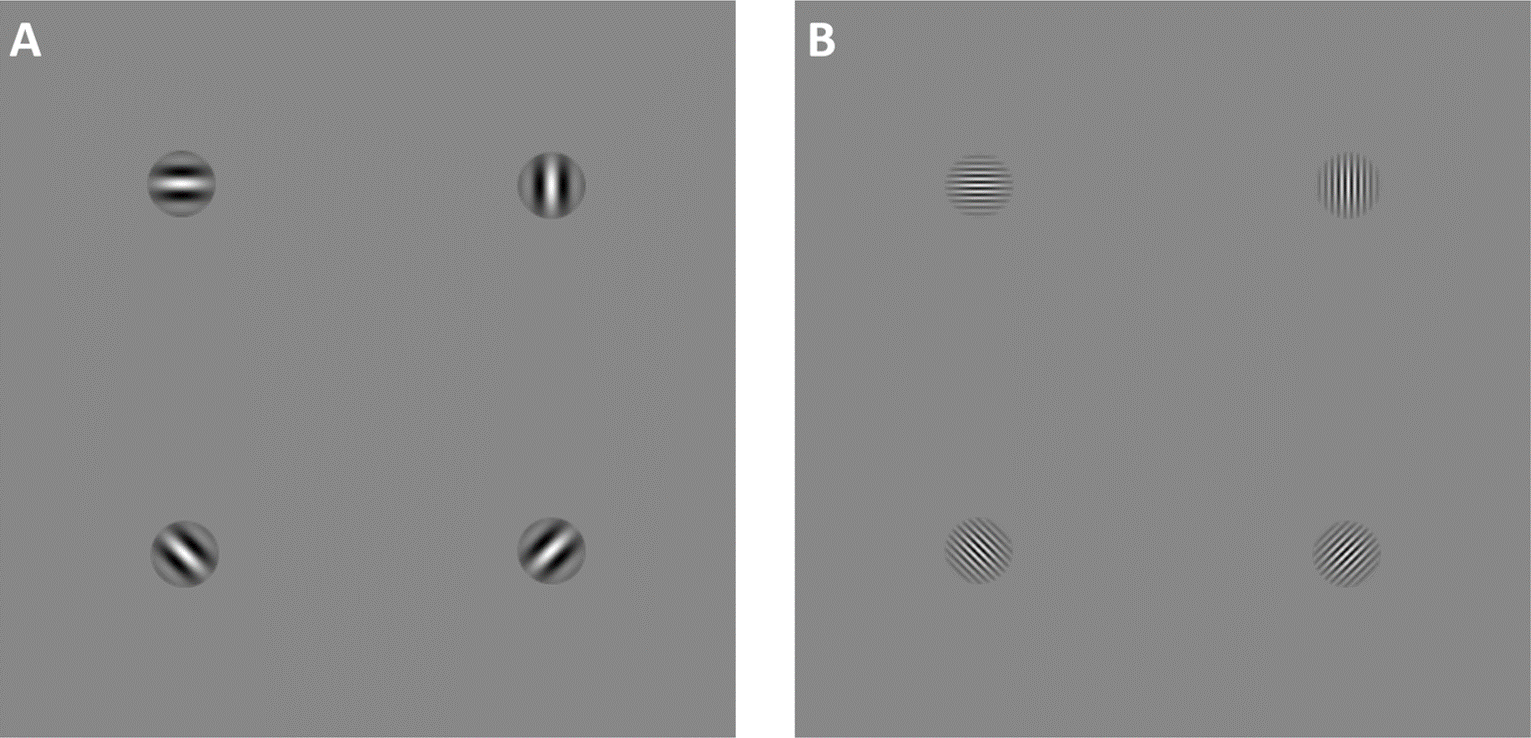
\includegraphics[width=\textwidth]{Figures/all_stimuli.png}
    \caption[Stimuli overview]{Stimuli overview. One stimulus has two varying conditions, the spatial frequency, which can either be low \textbf{A)}, at 2 cpd, or high \textbf{B)}, at 8 cpd. For each spatial frequency the Gabor patches can also vary between four orientations.}
    \label{fig:all_stimuli}
\end{figure}
\vspace{5mm}
\subsection{4 Alternative forced choice task}

In the 4 alternative forced choice task (4AFC) we presented the subjects with a stimulus of a random orientation and random spatial frequency. A proportion of 0.25 correct trials was the chance level and 0.625 was the perception threshold used in this analysis. In total there were 8 different stimulus conditions (Fig. \ref{fig:all_stimuli}). A rectangle was displayed in the center of the screen and the subject hat to fixate the center of that rectangle. In this rectangle the stimulus was presented. The stimuli appeared in a pseudo-randomized order, so that spatial frequency and orientation varied from trial to trial. Stimulus duration ranged from 16.6\,ms to 100\,ms (16.6, 33.3, 50, 66.6, 83.3 or 100\,ms). 

After the presentation of the stimulus an answer screen appeared (Fig. \ref{fig:answer_mask}). The answer buttons to choose the orientation alternated between two configurations. The mask in the center of the answer buttons was used to destroy the formation of an after image of the stimulus. The checkerboard corresponded to the spatial frequency of the previously presented stimulus. 
\begin{figure}[H]
    \centering
    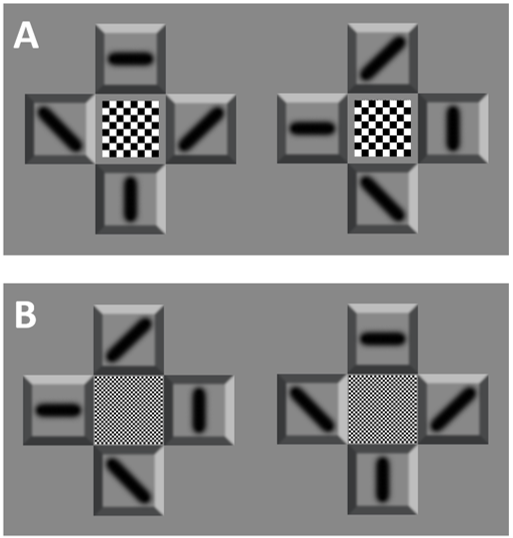
\includegraphics[scale = 0.5]{Figures/answer_mask.png}
    \caption[Answer mask]{Answer mask. After each stimulus presentation a mask surrounded by 4 answer buttons appeared on the screen.  The pattern of the checkerboard in the center corresponds to the low spatial frequency stimuli (\textbf{A}) or the high spatial frequency stimuli (\textbf{B}). For each spatial frequency there were two possible configurations of the answer buttons}
    \label{fig:answer_mask}
\end{figure}
\vspace{5mm}
The subject then had to choose the orientation it has seen out of the four possible orientations, if the orientation wasn't perceived confidently the subject had to choose randomly. The trial ended, when the subject clicked on of the answer buttons. A new trial started when the space bar was pressed. In total a subject had to complete 192 trials in a random order (2 stimulus conditions x 4 orientations x 6 presentation durations x\,4\,repetitions\,=\,192 trials).

Before the main experiment was started, the subject could familiarise themselves with the stimuli in a training protocol. In this protocol, each spatial frequency, stimulus condition, stimulus orientation and presentation duration was shown at least once. The subject could repeat this training until they felt comfortable with the protocol. 

\vspace{5mm}
\subsection{Comparative visual search task}

In the comparative visual search task (CVS) the subject had to compare two lists of stimuli and count the differences between them. One of the lists was always hidden behind a mask which moved with a varying delay. 

Each trial of the CVS task consisted of two columns (with a separation of 24 degrees of visual angle) with 12 stimuli each. The stimuli were the same as in the 4AFC task (Fig. \ref{fig:all_stimuli}). One list contained only Gabor patches one spatial frequency (spatial frequencies weren't mixed in a trial) but the order of the orientations of the Gabor patches was randomized. The stimulus configuration differed between the two lists at one, two or three random positions. A maximum of three differences was introduced to avoid premature trial completion, so that the subject had to go through the whole list. 
During all trials an opaque gray mask was visible which always covered one side of the screen so that only one list was
visible at all times. The corresponding positions were connected by a black line, that was visible at all times, even in the covered part of the screen. 
The subject could shift the mask from one side to the other via left and right mouse click to compare the two stimulus lists as often as desired.
One of two mask delays (0 or 2 seconds) were used and the order of used delays was randomized. The delay was initiated with the mouse click. During this mask delay, both columns remained hidden (Fig. \ref{fig:cvs_stimulus}). 
In total a subject had to complete 60 trials (2 spatial frequencies x 2 delays x 3 numbers of differences x 5\,repetitions\,=\,60). 
\begin{figure}[H]
    \centering
    \includesvg[width=\textwidth]{Figures/cvs methods.svg}
%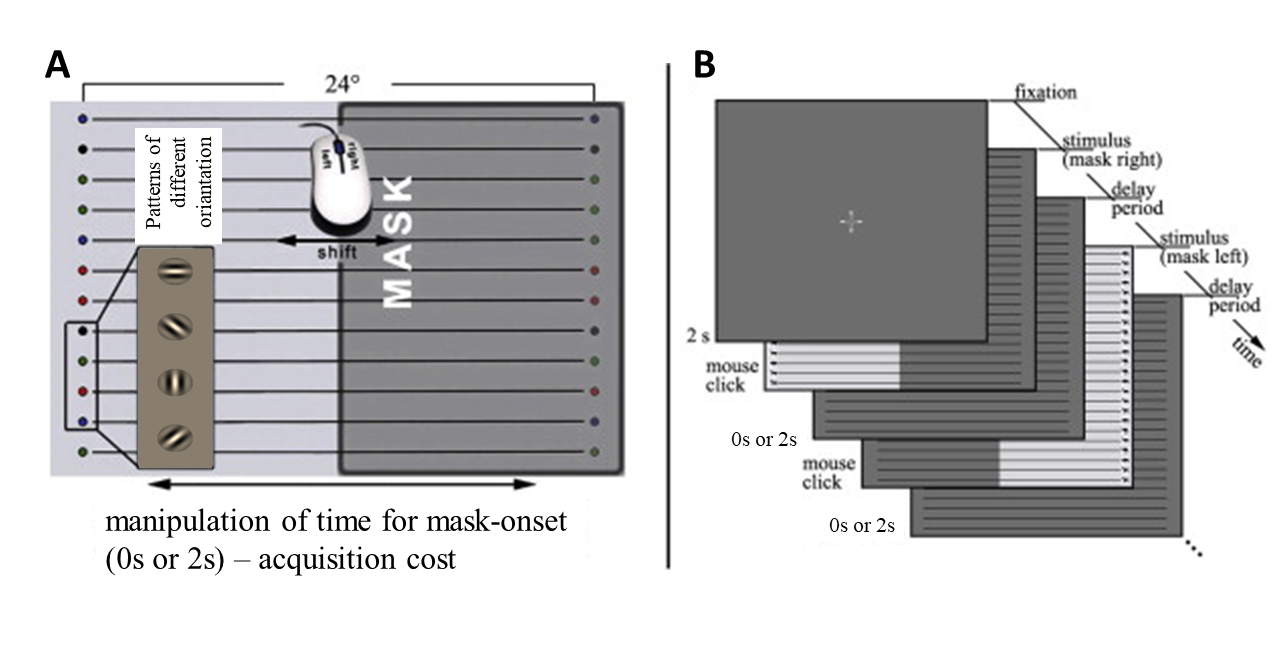
\includegraphics[width=\textwidth]{Figures/stimulus cvs methods.png}
    \caption[CVS stimulus]{Experimental paradigm. (\textbf{A}) Task setup. A stimulus image consists of two columns (column distance: 24°) with 12 items each. Items were Gabor patches of different orientation with either a low spatial frequency or a high spatial frequency (see Fig. \ref{fig:all_stimuli}). A gray opaque mask (shown here as transparent for sake of illustration) was always covering one column and could be shifted (to the other column) by clicking one of the two mouse buttons. The time for mask-onset after each click was manipulated by using one of the two mask delays. (\textbf{B}) Trial procedure. After presenting the fixation cross, the stimulus image appeared automatically with the right column covered. After clicking the left mouse button, the delay period started. Both columns of items were hidden during the time of delay and only the black lines were presented. The stimulus image reappeared after 0.0 or 2.0\,s with the left column covered. After clicking the right mouse button, the delay period started again. A trial was terminated by pressing the spacebar.}
    \label{fig:cvs_stimulus}
\end{figure}
The subjects’ task in each experimental trial was to compare the two lists of stimuli to find the number of differences (one, two or three) as quickly and reliably as possible.
After completion of the comparative search, space-bar had to be pressed to finish a trial. Afterwards, the identified number of differences had to be reported by clicking the corresponding number on the computer screen. 
During the fixation phase a fixation cross was displayed in the center of the screen for 1.5\,s. Next to the fixation cross the delay and the stimulus condition of the upcoming trial was displayed.
To get used to the stimulus presentation and the mouse controls, this task also included practice trials. In total there were four practice trials, one for each delay and stimulus condition combination. 
After this practise phase, the experiment started by
presenting the first trial. Subjects could take a break whenever they wanted but before they started a new trial. To avoid verbal rehearsal aiding in memorization during the delay phase, and thus adding an uncontrolled factor, these processes were articulatorily suppressed in all trials. To achieve this suppression, subjects had to repeatedly say out loud three irrelevant syllables (e.g., ‘bla-bli-blu’).


\vspace{5mm}
\subsection{Exclusion criteria}

Some data had to be excluded from our analysis, since some subjects showed performances that were either much worse than expected or much better. We can't ultimately exclude that software errors are responsible for these performances but assuming that it was the actual performance of the subjects we had to formulate criteria to either exclude or included these outlying performances. 

For the 4AFC task a subject had to perform at least at chance level (25\% correct) in at least 50\% of the presentation durations. Otherwise we assumed that stimuli either weren't perceived at all or the subject wasn't motivated to complete the task. 
We also excluded data of subjects when their detection threshold was outside of the presented range of presentation duration, since we can assume that in those cases the selected presentation durations didn't accurately reflect were the detection threshold of the subject might be.

For the CVS task we also implemented exclusion criteria to ensure that all subjects were motivated to complete the task. If in at least five of the 60 trials there were no switches in between the stimulus lists or the total duration was shorter than five seconds, we excluded the data from our analysis. 

\vspace{5mm}
\subsection{Analysis}
Data transformation as well as plotting where performed in Python 3.10 using the libraries Numpy, Scipy and Matplotlib. Statistical tests where conducted in Microsoft Excel. 

For the analysis of the 4AFC data we calculated the percentage of correct answers for each stimulus duration. We fitted a logistic function to the data of a single subject.
$$
P_{chance} + (1-P_{chance}) * \frac{1}{1+e^{-k(x -x_{0})}}
$$
Where the chance level $P_{chance} = 0.25$. The sigmoids midpoint $x_{0}$ as well as the logistic growth rate $k$ where optimized using the Trust Region Reflective algorithm to get the least squares. Using the fitted logistic function we computed the perception thresholds for every subject. All fits where visually inspected. Only perception thresholds within the presented stimulus ranges where used for subsequent analyses. The output of the stimulation software included trial number, number of differences, delay, cpd, reported differences, response time, number of switches and processing time. Processing time was calculated as the mean of all periods between two switches minus the delay duration.  

We conducted the analyses on the error rate of the answers, the response time (duration of one trial), the number of switches between the two columns and the processing time between two switches. Further, we constructed a strategy index

$$
S = \log_{10} \left( \frac{t_{p}}{n_{s}} \right)
$$

where $t_p$ is the processing time and $n_s$ the number of gaze shifts, both normalized between 0 and 1. The aim of the strategy index was to reduce the two dimensional strategy to a single dimension.

\vspace{5mm}
\subsection{Contrast sensitivity}

 We used the software "Kontrast.exe" to determine the contrast sensitivity curves for the three experimenters. This software presented a fixation point in the center of the screen and displayed gratings with a fixed spatial frequency but of varying contrast either on the left side or the right side of the fixation point for 100\,ms. The subject had to press the corresponding mouse button when they saw the grating (Left mouse button when the grating was perceived on the left side of the fixation point, right mouse button when the grating was perceived on the right side.) When no grating was perceived, the subject had to guess. The next stimulus was displayed immediately after the mouse click. To vary the spatial frequency in this experiment the subject had to complete on set of trials with a distance of 1\,m to the monitor resulting in a spatial frequency of 10 cpd of the grating, and in a second run of trials the distance was 2\,m resulting in a spatial frequency of 20 cpd. One run consisted of 180 trials (9 contrasts x 20 repetitions) so in total a subject had to complete 360 trials.

Analysis was done using MATLAB (version R2022a, MathWorks Ltd.) including the Psychophysics Toolbox extensions (Brainard, 1997). First the Michelson Contrast was calculated using  this formula:
\[
c = \frac{I\textsubscript{max}-I\textsubscript{min}}{I\textsubscript{max}+I\textsubscript{min}}
\]

With this formula we could calculate the contrast of each of the 9 stimulus condition. The presented Michelson contrasts ranged from 0 to 0.064. For the two-point-contrast calculations we also needed the averaged light intensities of the monitor calibration. This data was already measured for this exact monitor in a previous year. Now with the help of the Psychophysics Toolbox a logistic function was fitted the proportion of correct answers per stimulus condition. from this fit we could extract the perception threshold at 75\% for each subject. 

